\begin{figure}[ht!]
\centering

\scalebox{0.8}{
\begin{tikzpicture}[auto]

% operations =============================

\begin{scope}[xshift=0cm,yshift=0cm]
            \begin{scope}[xshift=0cm,yshift=0cm]
            \node (x1) at (1,1) {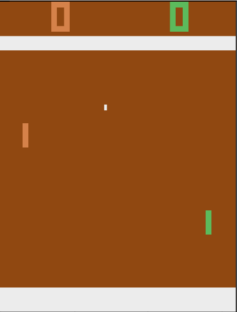
\includegraphics[width=.35\textwidth]{images/frame1.png}};
            \end{scope}
            \begin{scope}[xshift=-0.6cm,yshift=-0.6cm]
            \node (x2)  at (1,1) {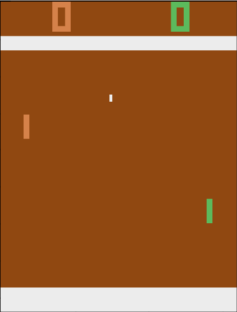
\includegraphics[width=.35\textwidth]{images/frame2.png}};
            \end{scope}
            \begin{scope}[xshift=-1.2cm,yshift=-1.2cm]
            \node (x3)  at (1,1) {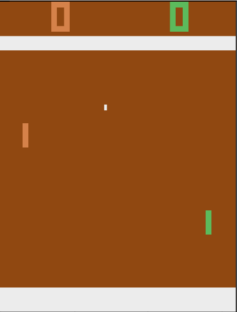
\includegraphics[width=.35\textwidth]{images/frame1.png}};
            \end{scope}  
\end{scope}


\node[textonly, right=10pt of x2] (inv1) {};
\node[op, right=60pt of x2] (f) {{\LARGE$f$}};
\node[textonly, right=2pt of f] (inv2) {};
\node[textonly, right=30pt of inv2] (result) {{\LARGE$\begin{bmatrix}Q(s,a_1)\\ \vdots \\Q(s,a_n)\end{bmatrix}$}};



%edges
\path[tedge, orange!120, line width=1.5mm]  (inv1) -- (f);
\path[tedge, orange!120, line width=1.5mm]  (inv2) -- (result);

\end{tikzpicture}
} % scalebox
\end{figure}